%%%%%%%%%%%%%%%%%%%%%%%%%%%%%%%%%%%%%%
% LaTeX poster template
% for Circuits and Systems 1 Project

\documentclass[final]{beamer}
\usepackage[scale=1.24]{beamerposter}
\usepackage{graphicx,subfigure,tikz,caption}			
\usetikzlibrary{positioning,arrows}
\setbeamertemplate{background canvas}{
  \begin{tikzpicture}
    \shade[top color=white,bottom color=white] (0,0) rectangle (\paperwidth,\paperheight);
  \end{tikzpicture}
}

\newlength{\sepwid}
\newlength{\onecolwid}
\newlength{\twocolwid}
\newlength{\threecolwid}
\setlength{\paperwidth}{48in}
\setlength{\paperheight}{36in}
\setlength{\sepwid}{0.024\paperwidth}
\setlength{\onecolwid}{0.22\paperwidth}
\setlength{\twocolwid}{0.464\paperwidth}
\setlength{\threecolwid}{0.708\paperwidth}
\setlength{\topmargin}{-0.5in}
\usetheme{confposter}
\usepackage{exscale}


\usecaptiontemplate{
\small
\structure{\insertcaptionname~\insertcaptionnumber:}
\insertcaption}

\setbeamercolor{block title}{fg=ngreen,bg=white}
\setbeamercolor{block body}{fg=black,bg=white}
\setbeamercolor{block alerted title}{fg=white,bg=dblue!70}
\setbeamercolor{block alerted body}{fg=black,bg=dblue!10}

\pgfdeclareimage[width=6in]{institute-logo}{UETlogo}
\logoleft{\pgfuseimage{institute-logo}\vspace*{-0.5cm}}

\pgfdeclareimage[height=12cm]{university-logo}{dcse_logo}
\logoright{\pgfuseimage{university-logo}}

%-----------------------------------------------------------
% Name and authors of poster/paper/research
%-----------------------------------------------------------

\title{Music-Reactive RGB LEDs Circuit}
\author{ Naveed Ahmad, Muhammad Kamil Khan, Sharjeel Qureshi }
\institute{Lab Instructor: Dr. Muniba Ashfaq\\ \vskip10pt
Course Instructor: Dr. Salman Ahmed \\ \vskip10pt
Course Lab: Circuits and System 1 Spring 2023}

%-----------------------------------------------------------
% Start the poster itself
%-----------------------------------------------------------


\begin{document}
\begin{frame}[t]

\begin{columns}[t]
\begin{column}{\sepwid}\end{column}
\begin{column}{\onecolwid}

% Introduction Block
\begin{block}{\textcolor{blue}{Introduction}}

\vskip1ex
\textbf{Introduction of the project}
\begin{itemize}
  \item A music-reactive RGB LED circuit combines RGB LEDs and audio input to create captivating light displays that synchronize with music.
  \item  The LEDs respond to sound levels and frequencies, producing dynamic lighting effects.
\end{itemize}
\vskip1ex
\end{block}

% Motivation Block
\vskip10ex
\begin{block}{\textcolor{purple}{Motivation}}

\begin{itemize}
\item \textbf{1: Party or Event Lighting:}
\begin{itemize}
\item Create an exciting atmosphere by synchronizing the LED lights with music at parties, concerts, or events. The dynamic lighting effects will enhance the overall experience and engage the audience.
\end{itemize}
\item \textbf{2: Home Entertainment:}
\begin{itemize}
\item Set up the circuit in your home entertainment area to elevate your movie-watching or gaming sessions. The LEDs will respond to the audio, adding a visual dimension and immersing you in the on-screen action.
\end{itemize}
\item \textbf{3: Mood Lighting:}
\begin{itemize}
\item Use the circuit as mood lighting in your living space or bedroom. The LED lights can change color and intensity based on the music you play, creating a relaxing or energizing ambiance according to your preference.
\end{itemize}
\item \textbf{4: Visual Performances:}
\begin{itemize}
\item Artists, DJs, and performers can incorporate the music-reactive LED circuit into their live performances. The synchronized lighting effects will captivate the audience and add a visual element to the music.
\end{itemize}
\item \textbf{5: Educational Demonstration:}
\begin{itemize}
\item The circuit can be utilized in educational settings to teach the principles of sound, electronics, and lighting. Students can learn about signal processing, amplification, and the interplay between audio and visual elements.
\end{itemize}
\end{itemize}
\end{block}

\vskip10ex
\end{column}

% The 2nd Column
\begin{column}{\sepwid}\end{column} % empty spacer column
\begin{column}{\twocolwid} % create a three-column-wide column and then we will split it up later
\begin{block}{\textcolor{red}{Circuit Schematic}}
\begin{figure}
  
  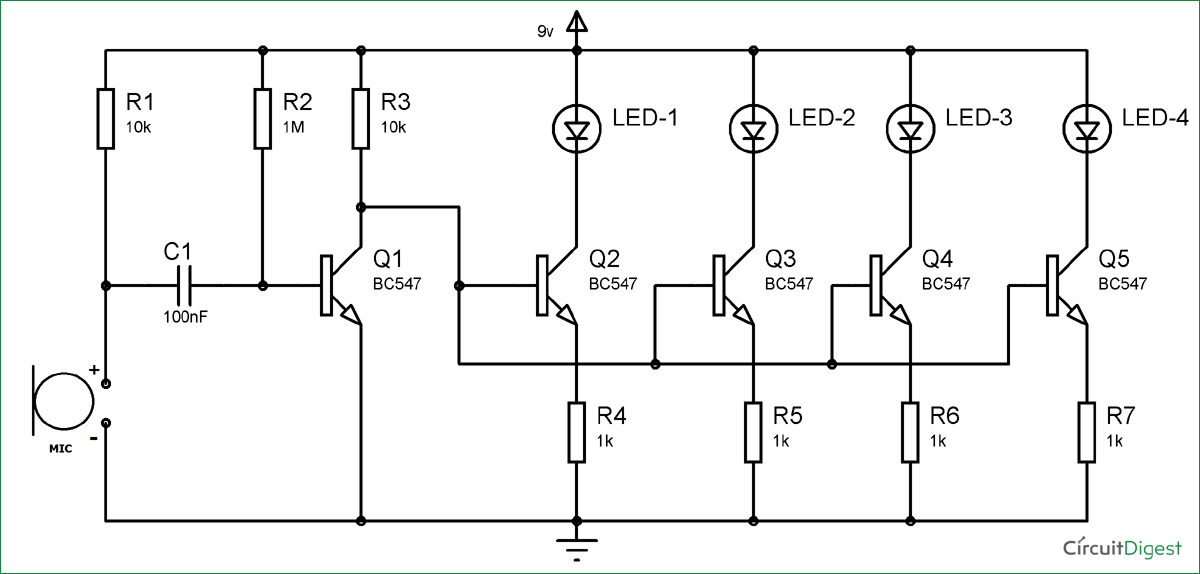
\includegraphics[scale=1.1]{image1.png}
  \caption{Schematic diagram}
  \label{fig:image1}
 \vspace{3cm}
   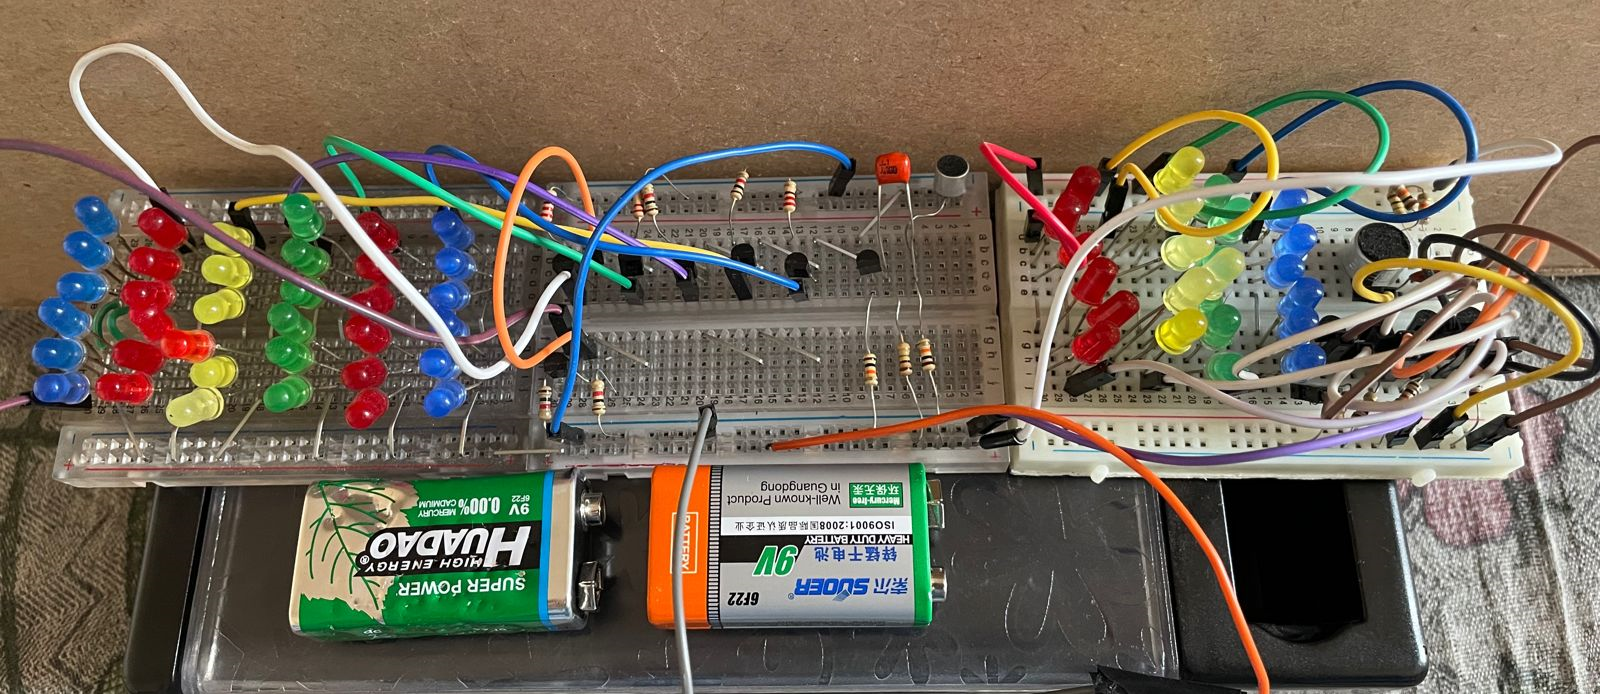
\includegraphics[scale=1.1]{PIC1.png}
  \caption{visual representation}
  \label{fig:image1}
\end{figure}
\end{block}
\end{column}

% Now is the last column
\begin{column}{\sepwid}\end{column} % empty spacer column
\begin{column}{\onecolwid}
\begin{block}{\textcolor{blue}{Operating Procedure}}


\begin{itemize}
\item \textbf{ Step 1: Sound Input:}
\begin{itemize}
  \item A condenser microphone captures sound signals and converts them into voltage levels.
  \item The microphone acts as a sensor that captures the
surrounding sound
\item The microphone converts sound signals into varying voltage
levels.
\end{itemize}

\begin{itemize}
\item \textbf{how Mic convert sound signal into voltage levels?}
\begin{itemize}
  \item The microphone consists of a diaphragm and a transducer.
\item Sound waves cause the diaphragm to vibrate, changing the
capacitance of the transducer.
\item The changing capacitance generates an electrical signal that
represents the sound.
\item The electrical signal from the microphone is in the form of
varying voltage levels corresponding to the sound waves.
\end{itemize}

\end{itemize}

\item \textbf{Step 2: Noise Filtering:}
\begin{itemize}
  \item A high-pass filter (resistor and capacitor) eliminates unwanted noise from the sound signals.
  \item This filter allows higher frequency components associated with
the music or sound to pass through while blocking lower frequency noise.

\end{itemize}
\item \textbf{Step 3: Signal Amplification:}
\begin{itemize}
  \item An NPN transistor amplifies the filtered signals.
  \item The transistor acts as an amplifier, boosting the strength of
the signals for further processing.
\end{itemize}
\item \textbf{Step 4: LEDs Activation:}
\begin{itemize}
  \item The amplified signals are fed into an array of transistors.
 \item Each transistor in the array acts as an amplifier as well.
 \item When the amplified signals pass through the transistors, they
trigger the corresponding LEDs to light up.
 \item Each transistor in the array works as an amplifier, causing the
 \item LEDs to glow based on the sound pattern.
 \item Additional LEDs can be added with transistors to enhance the
visual effect.
 \item Based on the analyzed data, the intensity or color of the RGB
LEDs changes, creating synchronized lighting effects
\end{itemize}
\end{itemize}

\end{block}

\end{column} % empty spacer column

\end{columns}
\end{frame}
\end{document}

